\documentclass[../../main/main.tex]{subfiles}
\graphicspath{{./figures/}}

\dominitoc
\faketableofcontents

\renewcommand{\mtcSfont}{\small\bfseries}
\renewcommand{\mtcSSfont}{\footnotesize}
\mtcsettitle{minitoc}{}
\mtcsetrules{*}{off}

\makeatletter
\renewcommand{\@chapapp}{Thermodynamique -- chapitre}
\makeatother

% \toggletrue{student}
\toggletrue{corrige}
% \renewcommand{\mycol}{black}
% \renewcommand{\mycol}{gray}

\hfuzz=5.003pt

\begin{document}
\setcounter{chapter}{4}

% \settype{book}
% \settype{prof}
% \settype{stud}

\chapter{Champs magnétiques}
% \epigraph{\openquote\textit{%
% 		Thermodynamics is a funny subject. The first time you go through it, you
% 		don't understand it at all. The second time you go through it, you think you
% 		understand it, except for one or two small points. The third time you go
% 		through it, you know you don't understand it, but by that time you are so
% 		used to it, it doesn't bother you anymore.
% 	}%
% 	\closequote}{Arnold \textsc{Sommerfeld}, $\approx$ 1950}

\vspace*{\fill}

\begin{tcn}*(appl)<ctc>{\iconsomm~Sommaire}
	\let\item\olditem
	\vspace{-15pt}
	\minitoc
	\vspace{-25pt}
\end{tcn}

\begin{tcn}*[fontupper=\small](appl)<ctb>"how"'t'{Capacités exigibles}
	\begin{itemize}[label=\rcheck]
		\item Exploiter une représentation graphique d’un champ vectoriel,
		      identifier les zones de champ uniforme, de champ faible et l’emplacement
		      des sources.

		\item Tracer l’allure des cartes de champs magnétiques pour un aimant droit,
		      une spire circulaire et une bobine longue.

		\item Décrire un dispositif permettant de réaliser un champ magnétique quasi
		      uniforme.

		\item Citer des ordres de grandeur de champs magnétiques : au voisinage
		      d’aimants, dans un appareil d’IRM, dans le cas du champ magnétique
		      terrestre.

		\item Exploiter les propriétés de symétrie et d’invariance des sources pour
		      prévoir des propriétés du champ créé.

		\item Évaluer l’ordre de grandeur d’un champ magnétique à partir
		      d’expressions fournies.

		\item Définir le moment magnétique associé à une boucle de courant plane.

		\item Associer à un aimant un moment magnétique par analogie avec une boucle
		      de courant.

		\item Citer un ordre de grandeur du moment magnétique associé à un aimant
		      usuel.
	\end{itemize}
\end{tcn}

\vspace*{\fill}

\newpage

\vspace*{\fill}
% {
% \begin{boxes}
\begin{tcn}[sidebyside, fontupper=\small, fontlower=\small](appl)<ctb>"check"'t'{L'essentiel}
	\begin{tcn}(defi)<ctc>'t'{Définitions}
		\tcblistof[\paragraph*]{defi}{\hspace*{4.8pt}}
	\end{tcn}
	% \begin{tcn}(rapp)<ctc>'t'{Rappels}
	% 	\tcblistof[\paragraph*]{rapp}{\hspace*{4.8pt}}
	% \end{tcn}
	\begin{tcn}(prop)<ctc>'t'{Propriétés}
		\tcblistof[\paragraph*]{prop}{\hspace*{4.8pt}}
		\tcblistof[\paragraph*]{loi}{\hspace*{4.8pt}}
		% \tcblistof[\paragraph*]{theo}{\hspace*{4.8pt}}
	\end{tcn}
	% \begin{tcn}(coro)<ctc>'t'{Corollaires}
	%   \tcblistof[\paragraph*]{coro}{\hspace*{4.8pt}}
	% \end{tcn}
	\begin{tcn}(demo)<ctc>'t'{Démonstrations}
		\tcblistof[\paragraph*]{demo}{\hspace*{4.8pt}}
		\tcblistof[\paragraph*]{prev}{\hspace*{4.8pt}}
	\end{tcn}
	% \begin{tcn}(inte)<ctc>'t'{Interprétations}
	% 	\tcblistof[\paragraph*]{inte}{\hspace*{4.8pt}}
	% \end{tcn}
	% \begin{tcn}(impl)<ctc>'t'{Implications}
	% 	\tcblistof[\paragraph*]{impl}{\hspace*{4.8pt}}
	% \end{tcn}
	% \begin{tcn}(tool)<ctc>'t'{Outils}
	% 	\tcblistof[\paragraph*]{tool}{\hspace*{4.8pt}}
	% \end{tcn}
	% \begin{tcn}(nota)<ctc>'t'{Notations}
	%   \tcblistof[\paragraph*]{nota}{\hspace*{4.8pt}}
	% \end{tcn}
	% \begin{tcn}(appl)<ctc>'t'{Applications}
	%   \tcblistof[\paragraph*]{appl}{\hspace*{4.8pt}}
	% \end{tcn}
	% \begin{tcn}(rema)<ctc>'t'{Remarques}
	%   \tcblistof[\paragraph*]{rema}{\hspace*{4.8pt}}
	% \end{tcn}
	% \begin{tcn}(exem)<ctc>'t'{Exemples}
	%   \tcblistof[\paragraph*]{exem}{\hspace*{4.8pt}}
	% \end{tcn}
	% \begin{tcn}*(ror)<ctc>"hart"'t'{Points importants}
	%   \tcblistof[\paragraph*]{ror}{\hspace*{4.8pt}}
	% \end{tcn}
	% \begin{tcn}(impo)<ctc>'t'{Erreurs communes}
	%   \tcblistof[\paragraph*]{impo}{\hspace*{4.8pt}}
	% \end{tcn}
	\tcblower
	% \begin{tcn}(defi)<ctc>'t'{Définitions}
	%   \tcblistof[\paragraph*]{defi}{\hspace*{4.8pt}}
	% \end{tcn}
	% \begin{tcn}(rapp)<ctc>'t'{Rappels}
	%   \tcblistof[\paragraph*]{rapp}{\hspace*{4.8pt}}
	% \end{tcn}
	% \begin{tcn}(prop)<ctc>'t'{Propriétés}
	%   \tcblistof[\paragraph*]{prop}{\hspace*{4.8pt}}
	%   \tcblistof[\paragraph*]{loi}{\hspace*{4.8pt}}
	%   \tcblistof[\paragraph*]{theo}{\hspace*{4.8pt}}
	% \end{tcn}
	% \begin{tcn}(coro)<ctc>'t'{Corollaires}
	%   \tcblistof[\paragraph*]{coro}{\hspace*{4.8pt}}
	% \end{tcn}
	% \begin{tcn}(demo)<ctc>'t'{Démonstrations}
	% 	\tcblistof[\paragraph*]{demo}{\hspace*{4.8pt}}
	% 	\tcblistof[\paragraph*]{prev}{\hspace*{4.8pt}}
	% \end{tcn}
	\begin{tcn}(inte)<ctc>'t'{Interprétations}
		\tcblistof[\paragraph*]{inte}{\hspace*{4.8pt}}
	\end{tcn}
	% \begin{tcn}(impl)<ctc>'t'{Implications}
	% 	\tcblistof[\paragraph*]{impl}{\hspace*{4.8pt}}
	% \end{tcn}
	% \begin{tcn}(tool)<ctc>'t'{Outils}
	%   \tcblistof[\paragraph*]{tool}{\hspace*{4.8pt}}
	% \end{tcn}
	% \begin{tcn}(nota)<ctc>'t'{Notations}
	%   \tcblistof[\paragraph*]{nota}{\hspace*{4.8pt}}
	% \end{tcn}
	\begin{tcn}(odgr)<ctc>'t'{Ordres de grandeur}
		\tcblistof[\paragraph*]{odgr}{\hspace*{4.8pt}}
	\end{tcn}
	% \begin{tcn}(appl)<ctc>'t'{Applications}
	% 	\tcblistof[\paragraph*]{appl}{\hspace*{4.8pt}}
	% \end{tcn}
	% \begin{tcn}(rema)<ctc>'t'{Remarques}
	%   \tcblistof[\paragraph*]{rema}{\hspace*{4.8pt}}
	% \end{tcn}
	% \begin{tcn}(exem)<ctc>'t'{Exemples}
	% 	\tcblistof[\paragraph*]{exem}{\hspace*{4.8pt}}
	% \end{tcn}
	\begin{tcn}*(ror)<ctc>"hart"'t'{Points importants}
		\tcblistof[\paragraph*]{ror}{\hspace*{4.8pt}}
	\end{tcn}
	\begin{tcn}(impo)<ctc>'t'{Erreurs communes}
		\tcblistof[\paragraph*]{impo}{\hspace*{4.8pt}}
	\end{tcn}
\end{tcn}
% \end{boxes}
% }%

\vspace*{\fill}
\newpage

\section{Introduction}
\subsection{Notion de champ en physique}
La notion de champ est omniprésente en physique.
\begin{tcb}(defi){Champ}
	Un \textbf{champ} est une grandeur physique définie en tout point M. Sa
	valeur dépend en général également du temps. Il peut être~:
	\begin{itemize}
		\setlength{\fboxsep}{3mm}
		\item[b]{Scalaire}: la grandeur physique est un scalaire (température,
		pression…). On l'écrit $\boxed{\psw{X (\Mr,t)}}$~;
		\item[b]{Vectoriel}: la grandeur physique est un vecteur (force,
		vitesse…). On l'écrit $\boxed{\psw{\vv{X}(\Mr,t)}}$~;
		\item[b]{Stationnaire}: la grandeur physique ne \textbf{dépend pas du
			temps}~: $\boxed{\psw{X (\Mr,\dcancel{t}) = X(\Mr)}}$~;
		\item[b]{Uniforme}: la grandeur ne \textbf{dépend pas de la position}~:
		$\boxed{\psw{X (\dcancel{\Mr},) = X(t)}}$.
	\end{itemize}
	% \begin{itemize}
	% 	\item Lorsque la grandeur physique est un scalaire (température,
	% 	      pression…), on parle de \textbf{champ scalaire}~: \psw{$X (\Mr,t)$~;}
	% 	\item Lorsqu'elle est un vecteur (force, vitesse…), on parle de
	% 	      \textbf{champ vectoriel}~: \psw{$\vv{X}(\Mr,t)$~;}
	% 	\item Lorsqu'elle ne dépend pas du temps, le champ est
	% 	      \textbf{stationnaire}~: $X (\Mr,\dcancel{t}) = X(\Mr)$~;
	% 	\item Lorsque la valeur ne dépend pas de la position dans l'espace, le
	% 	      champ est \textbf{uniforme}~: $X (\dcancel{\Mr},t) = X (t)$.
	% \end{itemize}
\end{tcb}
\begin{tcb}(exem)<lftt>'l'{Exemples}
	\begin{itemize}
		\item À deux dimensions, le champ d'altitude peut être défini sur une carte
		      de randonnée. En tout point $(x,y)$ de la carte, une grandeur $z(x,y)$ est
		      définie.
		\item On peut définir des champs de pression $p (x,y)$ ou de température
		      $T (x,y)$ sur une carte météorologique.
		\item On peut définir un champ de vitesse du vent $\vv{v}(x,y)$ où un vecteur
		      est défini en tout point d'une carte~: sa \textbf{direction} autant que sa
		      norme importent~;
		\item On peut aussi définir un champ de force gravitationnel $\Ff (x,y,z)$
		      dans tout l'espace, qui point toujours vers le centre de la Terre.
	\end{itemize}
\end{tcb}

\noindent
\begin{minipage}[t]{.5\linewidth}
	\centering
	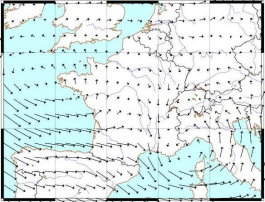
\includegraphics[scale=1]{champ_vent}
	\captionof{figure}{Champ vectoriel du vent en France.}
	\label{fig:chpvent}
\end{minipage}
\hfill
\begin{minipage}[t]{.5\linewidth}
	\centering
	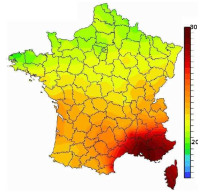
\includegraphics[scale=1]{champ_T}
	\captionof{figure}{Champ scalaire de la température en France.}
	\label{fig:chpT}
\end{minipage}

\subsection{Interaction entre aimants}
\textbf{Observations expérimentales}
\begin{itemize}
	\item Deux aimants peuvent s'attirer ou se repousser selon la façon dont on
	      les oriente~;
	\item Le champ magnétique peut être mis en évidence avec un petit aiment en
	      forme d'aiguille (boussole)~;
	\item Loin de toute perturbation, une aiguille s'oriente toujours sensiblement
	      dans la direction du sud vers le nord géographique.
\end{itemize}
\begin{tcb}(defi){Boussole}
	\begin{center}
		\psw{Une boussole est une aiguille aimantée libre de tourner.
			On appelle nord magnétique l'extrémité qui pointe vers le nord
			géographique.}
	\end{center}
\end{tcb}
Pour quantifier ces effets, on va introduire la notion de champ magnétique.

\subsection{Le vecteur champ magnétique}
La direction de l'aiguille aimantée en un point indique la direction du champ
magnétique.
\begin{tcb}(defi){Définition}
	\psw{Le \textbf{champ magnétique} est caractérisé par un
		\textbf{vecteur}, noté en général $\Bf$, tel que~:
		\begin{itemize}
			\item sa direction est celle d'une aiguille aimantée~;
			\item son sens va du pôle Sud au pôle Nord de l'aiguille~;
			\item sa norme s'exprime en tesla (\si{T}).
		\end{itemize}
	}
\end{tcb}

\section{Sources et cartes de champ magnétique}
\subsection{Aimant droit}
\label{ssec:aimdroit}
Un aimant possède un pôle nord \textbf{et} un pôle sud magnétique. Deux pôles de
même nature se repoussent, deux pôles de natures opposées se repoussent. Ceci
est dû à leur interaction magnétique, que l'on expliquera plus tard. Pour le
moment, nous nous contenterons de \textbf{représenter} le champ créé par un
aimant. Pour cela, plutôt que de représenter des flèches à chaque point de
l'espace autour d'un aimant (ce qui serait lourd), on utilise une représentation
plus légère~: les lignes de champ.
\begin{tcb}(defi){Définition}
	\psw{
		Les \textbf{lignes de champ} sont des courbes \textbf{orientées} tangentes
		en tout point au champ magnétique. Elles donnent la direction \textbf{et le
			sens} du champ magnétique en tout point.
	}
\end{tcb}

Pour visualiser un champ magnétique d'un aimant, on peut utiliser de la limaille
de fer. Les grains de limaille, de formes allongées, se transforment en petits
aimants sous l'action du champ magnétique~; ils se comportent ainsi comme de
petits boussoles qui s'orientent parallèlement au champ magnétique. On constate
que les grains de limaille forment des courbes particulières allant d'un pôle de
l'aimant vers l'autre, voir Figure~\ref{fig:lim1}.
\begin{figure}[h]
	\centering
	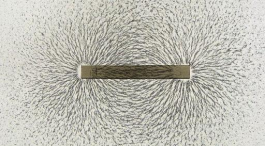
\includegraphics[scale=1]{lim1}
	\caption{Observation du champ magnétique d'un aimant au travers de son action
		sur l'orientation de grains de limaille de fer.}
	\label{fig:lim1}
\end{figure}
Ainsi, on observe la chose suivante~:
\begin{tcb}(prop){Propriété, heart}
	\psw{
		Les lignes de champ du champ magnétique sont des \textbf{courbes fermées}
		qui sortent de l'aimant par le pôle Nord et y rentrent par le pôle Sud.
	}
\end{tcb}
Schématiquement, on les représente de la manière suivante~:

\begin{figure}[h]
	\centering
	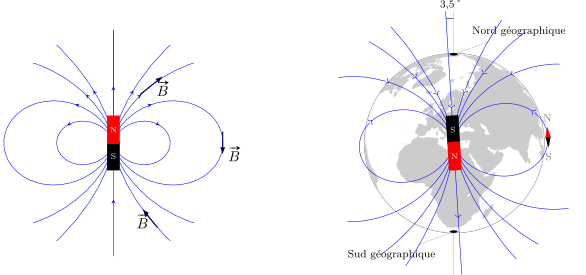
\includegraphics[scale=1]{aimdroit}
	\caption{Schématisation des lignes de champ dans un aimant droit, et
		schématisation du champ magnétique de la Terre comme celui d'un aimant droit.
		Une boussole à la surface de la Terre s'aligne sur le \textbf{pôle Sud magnétique}
		de la Terre, qui est proche du Nord géographique.}
	\label{fig:aimdroitterre}
\end{figure}

La Terre se comporte alors comme un gigantesque aimant. Son Sud magnétique se
situe au nord géographique, de sorte à ce que les nords magnétiques des
boussoles s'orientent vers le nord géographique.

\subsection{Champs magnétiques créés par des courants}
\label{ssec:chpcour}

En 1820, \textsc{Œrsted} découvre qu'un fil parcouru par un courant dévie une
aiguille aimantée~: c'est la première preuve historique qu'un courant électrique
créé un champ magnétique. De plus, en changeant le sens du courant, on change le
sens de l'aiguille. Regardons différentes manières de réaliser cette
expérience~:

\subsubsection{Bobine plate}
\label{sssec:bplate}
Une bobine plate est un fil électrique de forme circulaire. On refait une
expérience avec de la limaille de fer~: on retrouve alors des lignes qui sont
analogues à celles créées par l'aimant, si on le plaçait perpendiculairement à
la spire (ici, vertical).

\begin{figure}[h]
	\centering
	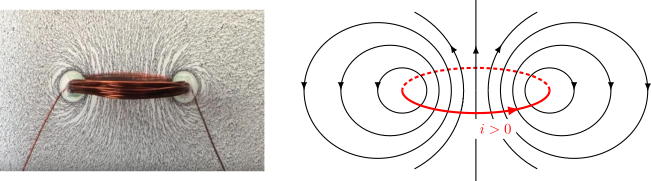
\includegraphics[scale=1]{bplate}

	\caption{Observation du champ créé par une bobine plate~: limaille de fer et
		schématisation.}
	\label{fig:bplate}
\end{figure}
Ainsi,
\begin{tcb}(prop){Comparaison aimant, hand}
	\begin{center}
		\psw{
			Les lignes de champ d'une bobine plate s'apparentent à celles d'un aimant
			droit.
		}
	\end{center}
\end{tcb}

\subsubsection{Solénoïde}
\label{sssec:solen}
\begin{tcb}(defi){Définition}
	\begin{center}
		\psw{
			En enroulant un fil le long d'un cylindre, on fabrique un
			\textbf{solénoïde}, ou bobine longue.
		}
	\end{center}
\end{tcb}

\noindent
\begin{minipage}[c]{.5\linewidth}
	\centering
	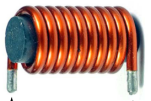
\includegraphics[scale=1]{sol_phot}
	\captionof{figure}{Photo d'un solénoïde.}
	\label{fig:solphot}
\end{minipage}
\hfill
\begin{minipage}[c]{.5\linewidth}
	\centering
	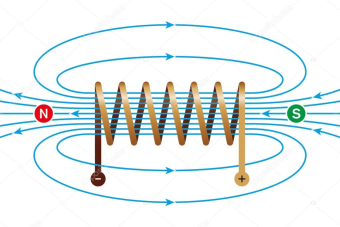
\includegraphics[width=\linewidth]{sol1}
	\captionof{figure}{Représentation d'un solénoïde avec lignes de champ.}
	\label{fig:sol1}
\end{minipage}

Étendre une bobine a pour effet de rendre les lignes de champ parallèles dans le
solénoïde. En dehors, les lignes de champ se referment de façon analogue encore
une fois à celle de l'aimant droit.

\section{Intensité du champ magnétique}
\label{sec:intchp}
\paragraph*{Expérience} Plus la boussole est proche de l'aimant, plus elle
s'aligne \textbf{rapidement} sur le champ magnétique. C'est au travers de ses
effets sur les courants, les aimants etc. que nous mesurons l'intensité du champ
magnétique, exprimé en tesla (\si{T}).
\begin{tcb}(exem)<lftt>'l'{OdGrangeurs}
	\begin{itemize}
		\item champ magnétique terrestre      $ \approx \SI{5e-5}{T} $~;
		\item champ créé par un aimant        $ \approx \SIrange{0.01}{0.5}{T} $~;
		\item champ créé par un électroaimant $ \approx \SIrange{1}{10}{T} $~;
		\item champ créé par un IRM           $ \approx \SI{10}{T} $~;
	\end{itemize}
\end{tcb}

\subsection{Lire une intensité sur une carte}
\paragraph*{Observation}
En reprenant l'exemple précédent du solénoïde, on remarque qu'une aiguille
s'alignera rapidement si elle est proche du solénoïde, voire à l'intérieur, mais
de plus en plus lentement quand on s'en éloigne. Ainsi,
\begin{itemize}
	\item l'intensité du champ décroît loin de la bobine~;
	\item les lignes de champ s'écartent les unes des autres.
\end{itemize}
Ces deux phénomènes sont tout à fait liés, et on a
\begin{tcb}(prop){Propriété, heart}
	\begin{center}
		\psw{
			\begin{itemize}
				\item Lignes de champ \textbf{proches} $\Lra$ champ intense~;
				\item Lignes de champ \textbf{éloignées} $\Lra$ champ moins intense~;
				\item Lignes de champ \textbf{parallèles} $\Lra$ champ uniforme.
			\end{itemize}
		}
	\end{center}
\end{tcb}

\subsection{Dispositifs créant un champ uniforme}
On a trois manière aisées de créer un champ uniforme~:
\begin{enumerate}
	\item Dans un solénoïde, les lignes de champ sont parallèles, c'est une
	      première façon~;
	\item Entre les deux pôles d'un aimant en U, l'expérience avec la limaille de
	      fer montre que le champ est uniforme (voir Figures~\ref{fig:aimu_lim}
	      et~\ref{fig:aimu_sch}).
	      \smallbreak
	      \noindent
	      \begin{minipage}[c]{.45\linewidth}
		      \centering
		      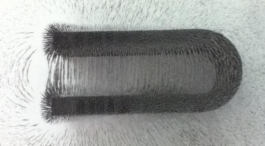
\includegraphics[scale=1]{aimu_lim}
		      \captionof{figure}{Observation du champ magnétique dans un aimant en
			      U par limaille de fer.}
		      \label{fig:aimu_lim}
	      \end{minipage}
	      \hfill
	      \begin{minipage}[c]{.45\linewidth}
		      \centering
		      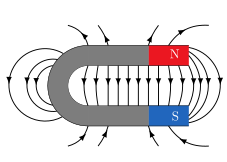
\includegraphics[scale=1]{aimu_sch}
		      \captionof{figure}{Schématisation du champ magnétique dans un aimant en
			      U.}
		      \label{fig:aimu_sch}
	      \end{minipage}
	\item On peut également créer un champ magnétique uniforme avec deux bobines
	      plates dans une configuration particulière~: deux bobines de rayon $R$ et
	      \textbf{disposées à une distance $R$ l'une de l'autre}, si elles sont
	      parcourues par la même intensité, donnent un champ magnétique uniforme entre
	      elles. On appelle cet ensemble une \textbf{bobine de \textsc{Helmoltz}}~;
	      voir Figure~\ref{fig:helm}.
	      Vous pourrez pour cela manipuler une animation disponible en
	      ligne\footnote{\url{www.sciences.univ-nantes.fr/sites/genevieve_tulloue/Elec/Champs/Helmholtz_FJ.php}}.
\end{enumerate}
\begin{figure}[h]
	\centering
	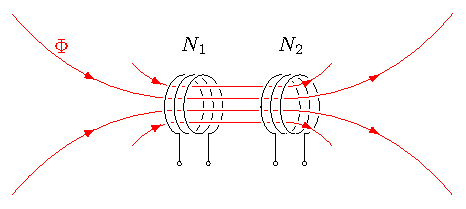
\includegraphics[width=.7\linewidth]{helmoltz}
	\caption{Représentation des lignes de champ d'une bobine de \textsc{Helmoltz}.
		Le schéma n'est pas exactement à l'échelle~: il faut que la distance entre les
		bobines soit égale à leur rayon.}
	\label{fig:helm}
\end{figure}

\subsection{Lien entre courant et champ magnétique}
\label{ssec:lienicour}
\subsubsection{Direction du champ magnétique}
\label{sssec:chpdir}
\begin{tcb}(prop){Règles de la main droite, heart}
	\begin{minipage}[t]{.45\linewidth}
		\begin{center}
			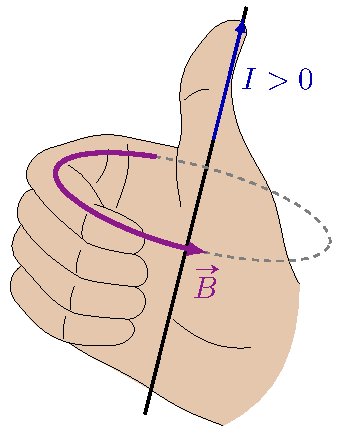
\includegraphics[width=.5\linewidth]{ra_fil}
			\label{fig:rafil}
			\captionof{figure}{Pour un champ créé par un fil~: pouce sur le courant,
				doigts selon $\protect\Bf$.}
		\end{center}
	\end{minipage}
	\hfill
	\begin{minipage}[t]{.45\linewidth}
		\begin{center}
			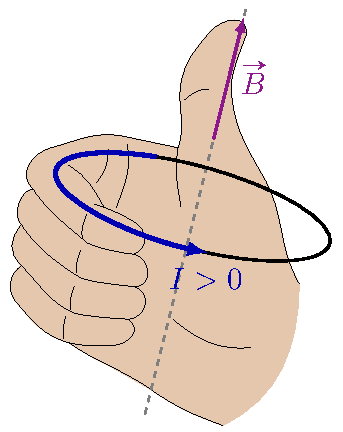
\includegraphics[width=.5\linewidth]{ra_bob}
			\label{fig:rabob}
			\captionof{figure}{Pour un champ créé par une bobine~: pouce sur
				$\protect\Bf$, doigts selon le courant.}
		\end{center}
	\end{minipage}
\end{tcb}
\begin{tcb}(exem)<lftt>'l'{Application}
	\centering
	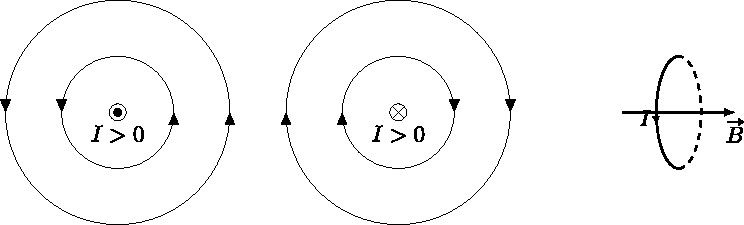
\includegraphics[scale=1]{ra_app}
\end{tcb}

\subsubsection{Proportionnalité}
\label{sssec:prop}
Dans le vide, le champ magnétique créé par un courant $i$ est de l'ordre de~:
\[
	\norm{\Bf} = \mu_0 \frac{i}{L}
\]
avec~:
\begin{itemize}
	\item $i (t)$ le courant~;
	\item $\mu_0 = 4\pi\cdot \SI{e-7}{H.m ^{-1}}$ est la \textbf{perméabilité du
		      vide}~;
	\item $L$ est une longueur typique du système.
\end{itemize}
Par exemple, à l'intérieur d'un solénoïde où le champ est uniforme, on a
\[
	\Bf = \mu_0ni (t)\uz
\]
avec $\uz$ l'axe du solénoïde orienté selon la règle de la main droite par
rapport au courant, et $n$ le nombre de spires par mètre.

\subsubsection{Symétries de la distribution de courant}
\label{sssec:symdist}
Les situations qu'on a étudiées jusque-là ont toutes fait preuve d'une certaine
symétrie, et ce n'est pas un hasard. L'étude des symétries est d'ailleurs toute
une science en soit, qui a mené à une des plus grandes découvertes scientifiques
du monde~: le théorème de \textsc{Noether}\footnote{Figure incontournable de la
	physique moderne, Emmy \textsc{Noether} était une mathématicienne hors pair,
	reconnue dans le monde scientifique à une époque où les femmes étaient encore
	plus minimisées qu'aujourd'hui. \textsc{Einstein} aurait qualifié son théorème
	de «~monument de la pensée mathématique~».}, démontré en 1915. Contentons-nous
de géométrie pour le moment…
\begin{tcb}(ror){Symétries, hand}
	Soit M un point, $\mathcal{P}$ un plan de symétrie de la distribution, et
	$\mathcal{P'}$ un plan d'\textbf{anti}symétrie. Alors~:
	\psw{
		\begin{itemize}
			\item $\Mr \in \mathcal{P} \Lra \vv{B}(M) \perp \mathcal{P}$~;
			\item $\Mr \in \mathcal{P'} \Lra \vv{B}(M) \in \mathcal{P'}$.
		\end{itemize}
	}
\end{tcb}
\begin{tcb}(exem){Exemples}
	\begin{enumerate}
		\item Soit un fil doté de coordonnées cylindriques.
		      \begin{center}
			      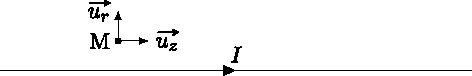
\includegraphics[scale=1]{sym1}
		      \end{center}
		      \psw{
			      \begin{itemize}[label=$\diamond$, leftmargin=20pt]
				      \item $\mathcal{P'} = (\Mr,\ur,\ut)$ est plan de d'\textbf{anti}symétrie
				            (si on fait le miroir du courant il va dans le sens opposé), donc
				            $\vv{B} \in \mathcal{P}$.
				      \item $\mathcal{P} = (\Mr,\ur,\uz)$ est plan de \textbf{symétrie}~:
				            $\vv{B} \perp \mathcal{P} \Ra \vv{B} \parr \ut$.
			      \end{itemize}
		      }
		\item Soit un solénoïde avec des coordonnées cylindriques.
		      \begin{center}
			      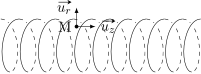
\includegraphics[scale=1]{sym2}
		      \end{center}
		      \psw{
			      \begin{itemize}[label=$\diamond$, leftmargin=20pt]
				      \item $\mathcal{P} = (\Mr,\ur,\ut)$ plan de \textbf{symétrie}~:
				            $\vv{B} \perp \mathcal{P} \Ra \vv{B} \parr \uz$.
			      \end{itemize}
		      }
	\end{enumerate}
\end{tcb}
\subsubsection{Invariances de la distribution de courants}
\label{sssec:invdist}
\begin{tcb}(ror){Invariances, hand}
	\begin{center}
		\psw{
			Le champ $\vv{B}$ possède les mêmes \textbf{invariances} que la
			distribution de courant
		}
		\vspace{12pt}
		\smallbreak
		\textbf{Attention}~: il ne faut pas confondre symétrie et invariance~!
	\end{center}
	\begin{minipage}[]{.45\linewidth}
		\begin{center}
			\fbox{\textbf{Symétrie}}
		\end{center}
		\textbf{Spécifique} à chaque champ, dépend d'un \textbf{plan miroir} de la
		distrubution, donne la \textbf{direction}.
	\end{minipage}
	\hfill
	\begin{minipage}[]{.45\linewidth}
		\begin{center}
			\fbox{\textbf{Invariance}}
		\end{center}
		\textbf{Général}, dépend d'une \textbf{translation} ou \textbf{rotation} de
		la distribution, donne la dépendence aux \textbf{coordonnées}.
	\end{minipage}
\end{tcb}

\begin{tcb}(exem)<lftt>'l'{Exemple}
	\begin{enumerate}
		\item Pour un fil infini par exemple, le translater selon $z$ ne change pas
		      la distribution. Il n'y a donc aucune raison que $\vv{B}$ dépende de $z$.
		\item De la même manière, pour tout fil parcouru par un courant, on a
		      invariance de la distribution par rotation selon $\theta$~: $\vv{B}$ ne
		      saurait dépendre de $\theta$.
	\end{enumerate}
	Autrement dit, par l'étude des invariances pour un fil infini, on
	sait que
	\[
		\vv{B}(r,\dcancel{\theta},\dcancel{z})
	\]
	Si on ajoute l'étude des symétries, on a que $\vv{B}\parr \ut$. Tout combiné,
	on a donc
	\[
		\boxed{\vv{B}(\Mr) = B(r)\ut}
	\]
\end{tcb}

\subsection{Exercice bilan}
\label{ssec:bilandir}
Les cartes de champ magnétique ci-dessous sont des vues en coupe du champ
produit par des spires de courant circulaires. Dans les deux cas, indiquer 1/ la
position des sources, 2/ le sens du courant circulant dans les spires, 3/ les
zones de champ fort et faible, et 4/ le cas échéant s'il existe une zone de
l'espace où le champ magnétique est uniforme.
\begin{figure}[h]
	\centering
	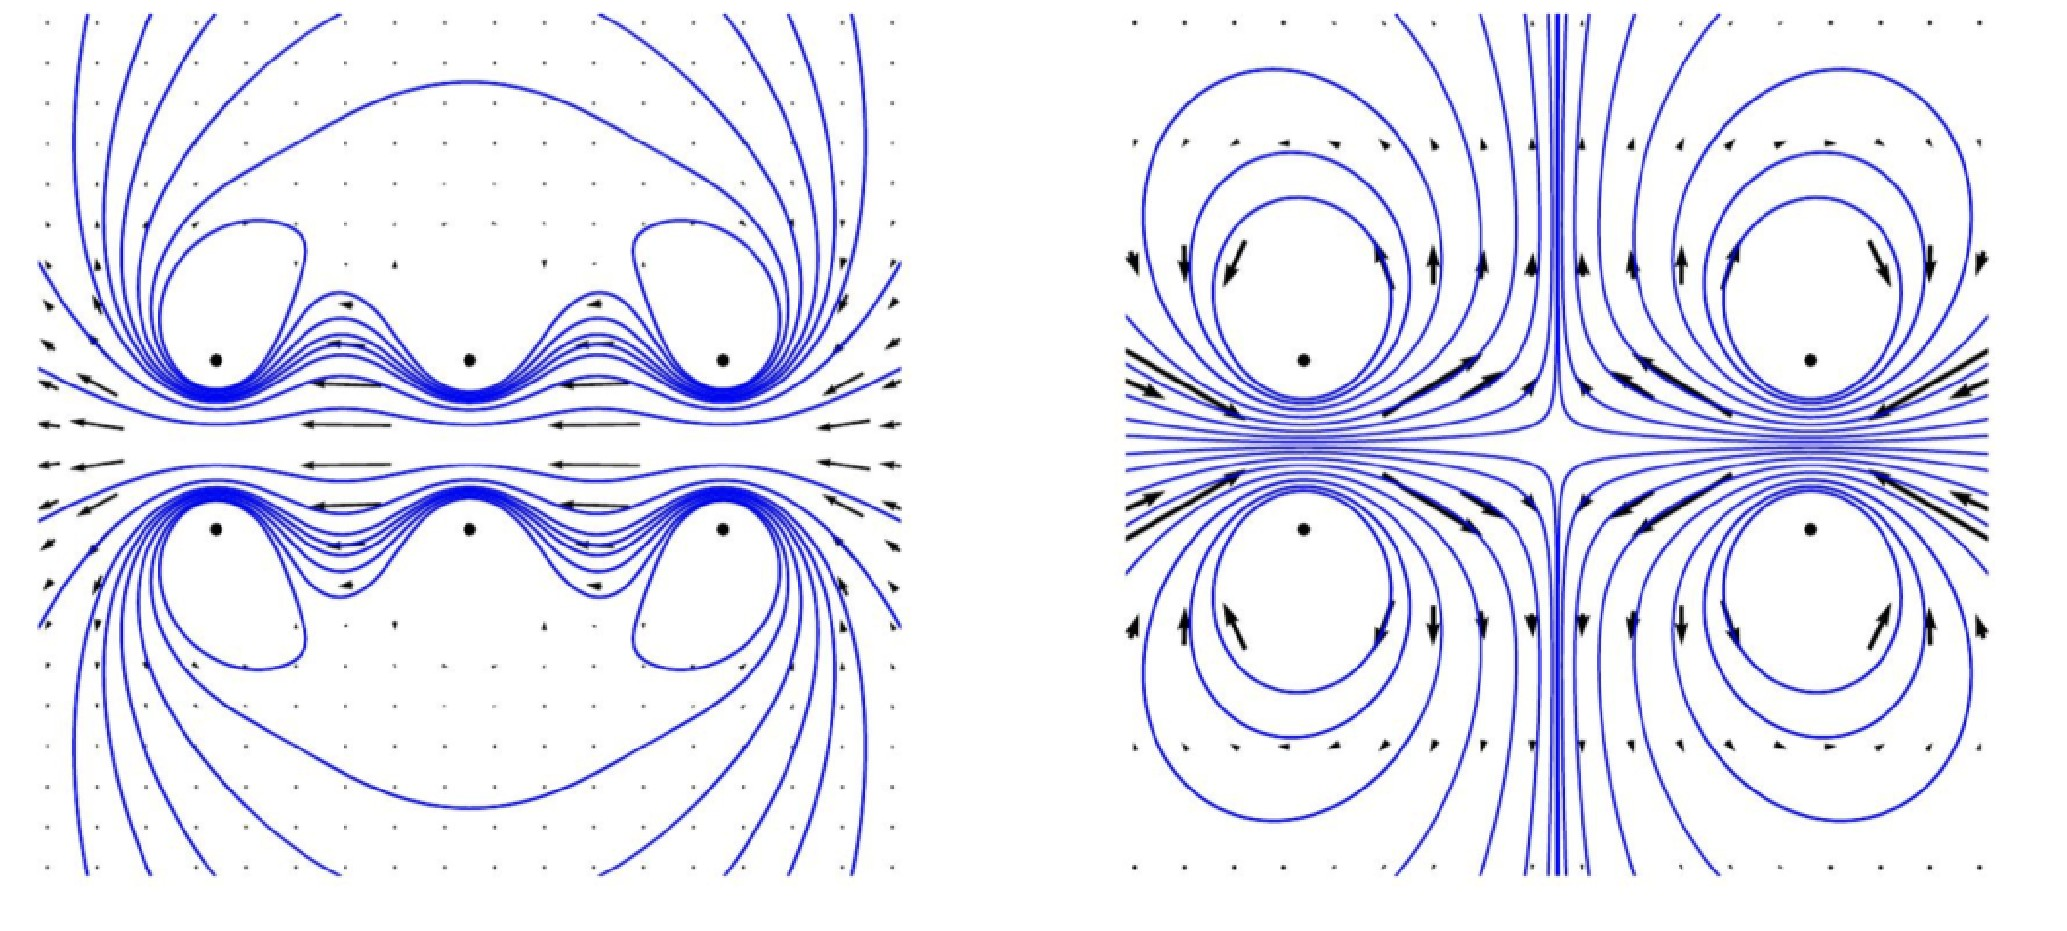
\includegraphics[scale=.8]{ldc_bilan}
	\caption{Représentation des lignes de champ pour différentes situations avec
		des pires de courant.}
	\label{fig:ldc_bilan}
\end{figure}

\vspace*{-10pt}

\section{Le moment magnétique}
\label{sec:momag}
\subsection{Boucle de courant}
\label{ssec:magboucle}
\begin{tcb}(defi){Définition, heart}
	\begin{minipage}[t]{.48\linewidth}
		\psw{
			On considère une spire de rayon $R$ parcourue par un courant $i$. La normale à
			la surface est notée $\vv{n}$, orientée dans le sens de la main droite par
			rapport au courant.
			\smallbreak
			Le \textbf{moment magnétique} $\vv{\mu}$ de la spire plane est
			\[
				\boxed{\vv{\mu} = i \vv{S} = i\pi R^2 \vv{n}}
			\]
			avec $\vv{S} = \pi R^2 \vv{n}$ le vecteur surface, en \si{m^2}~: le moment
			magnétique s'exprime donc en \fbox{\si{A.m^{2}}}.
		}
	\end{minipage}
	\hfill
	\begin{minipage}[t]{.48\linewidth}
		~
		\vspace{0pt}
		\begin{center}
			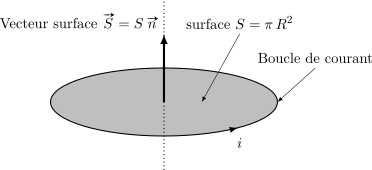
\includegraphics[width=\linewidth]{momag}
			\label{fig:momag}
		\end{center}
	\end{minipage}
\end{tcb}

Dans ce cas, c'est le mouvement de \textbf{particules chargées} qui créé le
champ magnétique. Cette notion s'applique également aux bobines.

\subsection{Cas des aimants}
\label{ssec:magaim}
La notion de moment magnétique s'applique aussi aux aimants, même si sa source
n'est pas due à un mouvement de translation comme peut l'être le courant dans un
fil~: la source du magnétisme dans les aimants est intrinsèquement
\textbf{quantique}, et vient de la nature aimantée des électrons. Ce sont
ensuite des effets à grande échelle qui permettent l'existence d'un champ à
l'échelle d'un solide entier.

\begin{tcb}(exem)<lftt>'l'{OdG}
	On a comme ordre de grandeur~: aimant droit $\approx \SI{1}{A.m^2}$~; aimant
	néodyme $\approx \SI{10}{A.m^2}$~; pour la Terre $\approx \SI{8e22}{A.m^2}$.
\end{tcb}

\end{document}
